\noindent Bằng cách sử dụng quang phổ tia X và phổ quang điện tử, ta có thể thu được thông tin về cấu trúc của vật chất. Sơ đồ bố trí thiết bị thí nghiệm được chỉ ra trong hình 8. Ống tia X bao gồm một cathode của súng điện tử và một anode kim loại. Các electron phát ra từ cathode sẽ được tăng tốc bởi điện áp, sau đó va chạm với anode kim loại để tạo ra tia X (không tính đến bức xạ trước khi electron va chạm với anode). Phổ của nó bao gồm phổ liên tục của bức xạ hãm và phổ đặc trưng rời rạc. Trong thí nghiệm, người ta sử dụng tia X có bước sóng nhất định để tương tác với bia vật liệu, sau đó sử dụng đầu thu quang phổ tia X và đầu thu phổ quang điện tử để phát hiện tia X và quang điện tử phát ra.
\newpage

\begin{figure}[h]
  \centering
  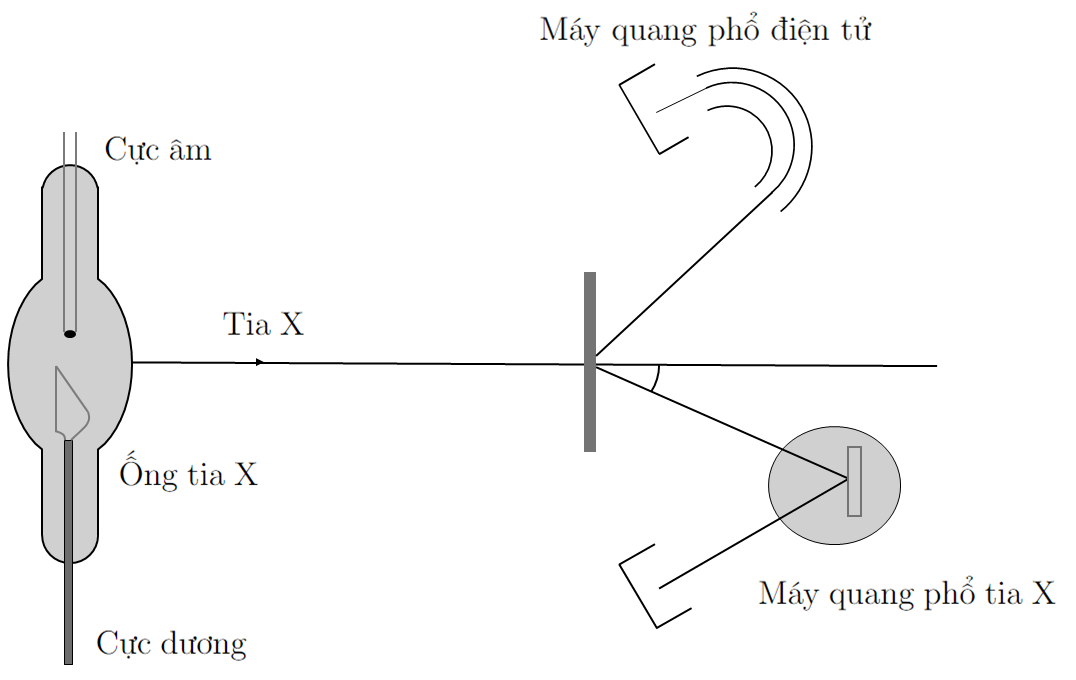
\includegraphics[width=0.65\textwidth]{images/Hinh 8a.png}
  \begin{center}
    \figurename{ 8a: Sơ đồ bố trí thí nghiệm.}
  \end{center}
\end{figure}

\begin{figure}[h]
  \centering
  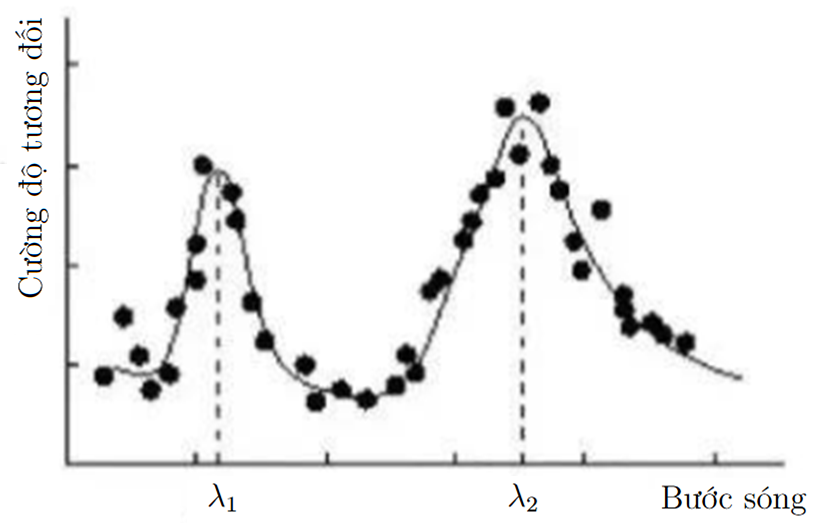
\includegraphics[width=0.58\textwidth]{images/Hinh 8b.png}
  \begin{center}
    \figurename{ 8b: Quang phổ tia X.}
  \end{center}
\end{figure}

\noindent Biết hằng số Rydberg $R_{\infty}=$\SI{10973731}{\metre^{-1}}, $hc=$\SI{1240}{\nano\metre\electronvolt} trong đó $h$ và $c$ lần lượt là hằng số Plank và vận tốc ánh sáng trong chân không.
\begin{enumerate}
  \item Lý thuyết Bohr có thể lý giải các mức năng lượng và phổ của nguyên tử Hydrogen hoặc hệ ion hoá giống Hydrogen. Năng lượng và trạng thái của electron trong hệ phụ thuộc vào số lượng tử $n$. Đối với hệ nguyên tử gồm nhiều electron, electron trong nguyên tử có thể được chia thành các lớp vỏ $K(n=1), L(n=2)$ và $M(n=3)$ tuỳ thuộc vào giá trị của $n$. BIết rằng năng lượng của electron trong lớp $K$ của nguyên tử kim loại ở anode là \SI{-20,1}{\kilo\electronvolt}.
        \begin{enumerate}
          \item[a.] Xác định điện áp tối thiểu cần sử dụng để ion hoá một electron trong lớp vỏ $K$ của nguyên tử kim loại, từ đó gây ra sự chuyển dịch mức năng lượng của electron từ lớp $L$ về lớp $K$ và phát ra tia X. Kết quả làm tròn đến ba chữ số thập phân.
          \item[b.] Với điện áp tính được ở ý a, bước sóng ngắn nhất của tia X phán ra từ ống tia X là bao nhiêu? Kết quả làm tròn đến ba chữ số thập phân.
          \item[c.] Nếu năng lượng của photon tia X đặc trưng $K_{\alpha}$ phát ra từ nguyên tử kim loại là \SI{17,44}{\kilo\electronvolt}, hãy xác định số điện tích hạt nhân của nguyên tử này.
        \end{enumerate}
  \item Sử dụng tia X đặc trưng $K_{\alpha}$ có bước sóng $\lambda$ tác động vào một bia vật liệu, giả sử electron trong bia vật liệu ở trạng thái tĩnh và có khối lượng nghỉ là $m$. Biết góc tán xạ (góc giữa tia X tán xạ và tia X tới) là $\theta$. Hãy tìm bước sóng của tia X tán xạ và động năng của electron quang điện tử.
  \item Trong thí nghiệm, phổ tán xạ đo được tại góc $\theta=135^{\circ}$. Hình 8b cho thấy có hai đỉnh phổ ứng với các bước sóng $\lambda_{1}$ và $\lambda_{2}$. Giải thích nguồn gốc hai đỉnh phổ này và nguyên nhân khiến cho độ rộng của đỉnh phổ $\lambda_{1}$ lớn hơn độ rộng của đỉnh phổ $\lambda_{2}$.
\end{enumerate}